\documentclass{article}
\usepackage{graphicx}
\usepackage[margin=1.5cm]{geometry}
\usepackage{amsmath}

\begin{document}

\title{Thursday Reading Assessment: Chapter 4}
\author{Prof. Jordan C. Hanson}

\maketitle

\begin{figure}[ht]
\centering
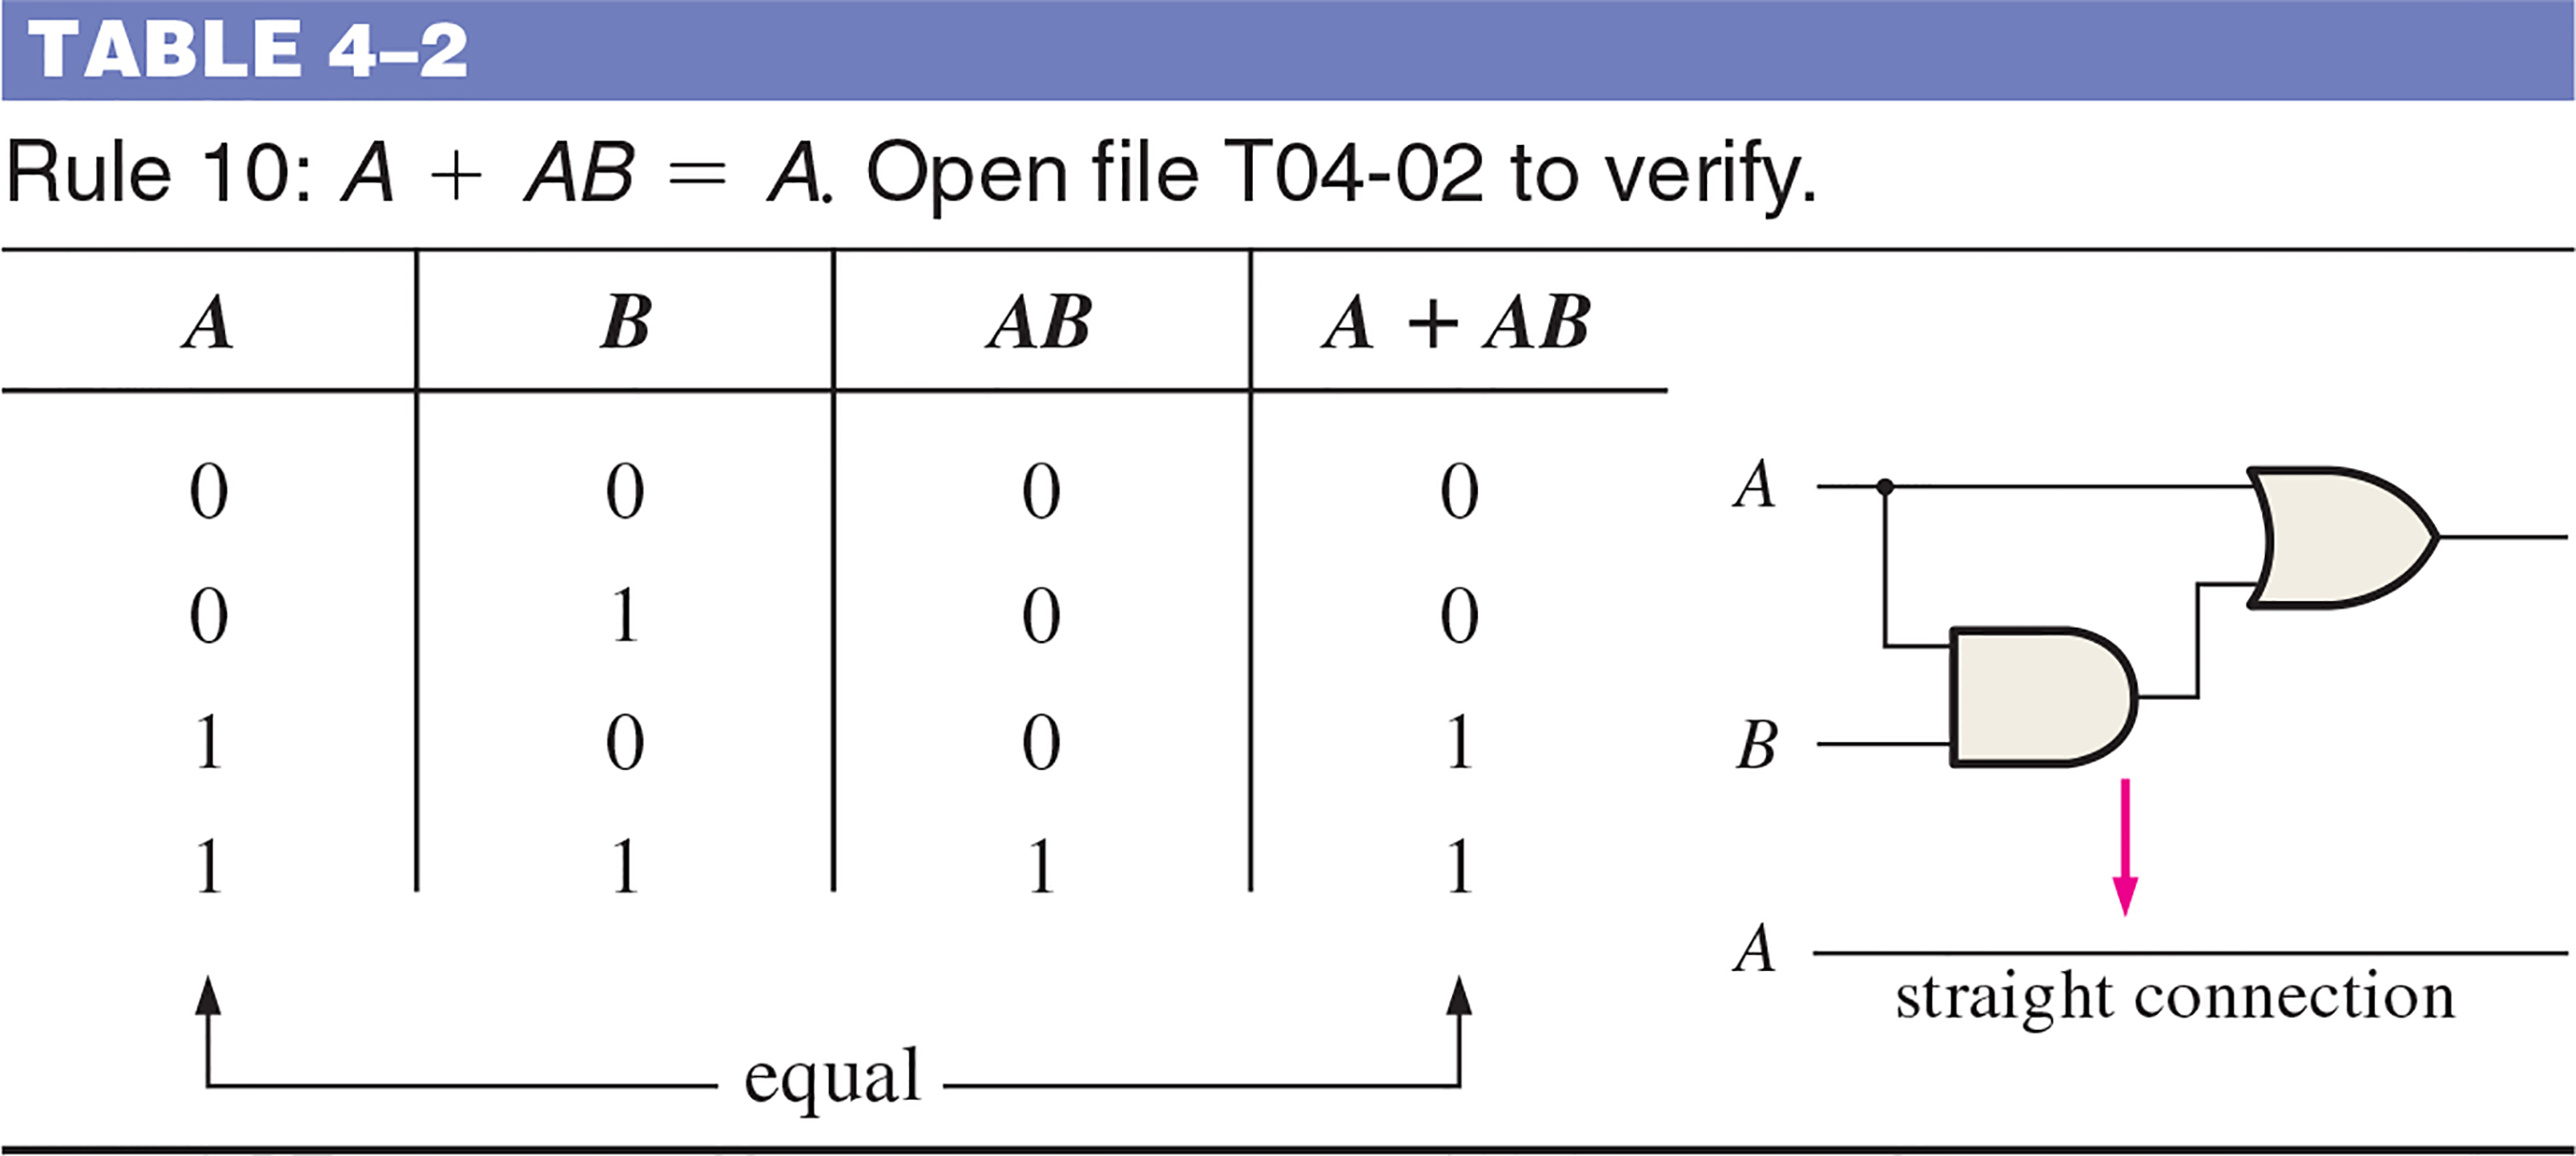
\includegraphics[width=0.25\textwidth,trim=15cm 1cm 0cm 3cm,clip=true]{figures/AND_OR.jpg} \hspace{0.5cm}
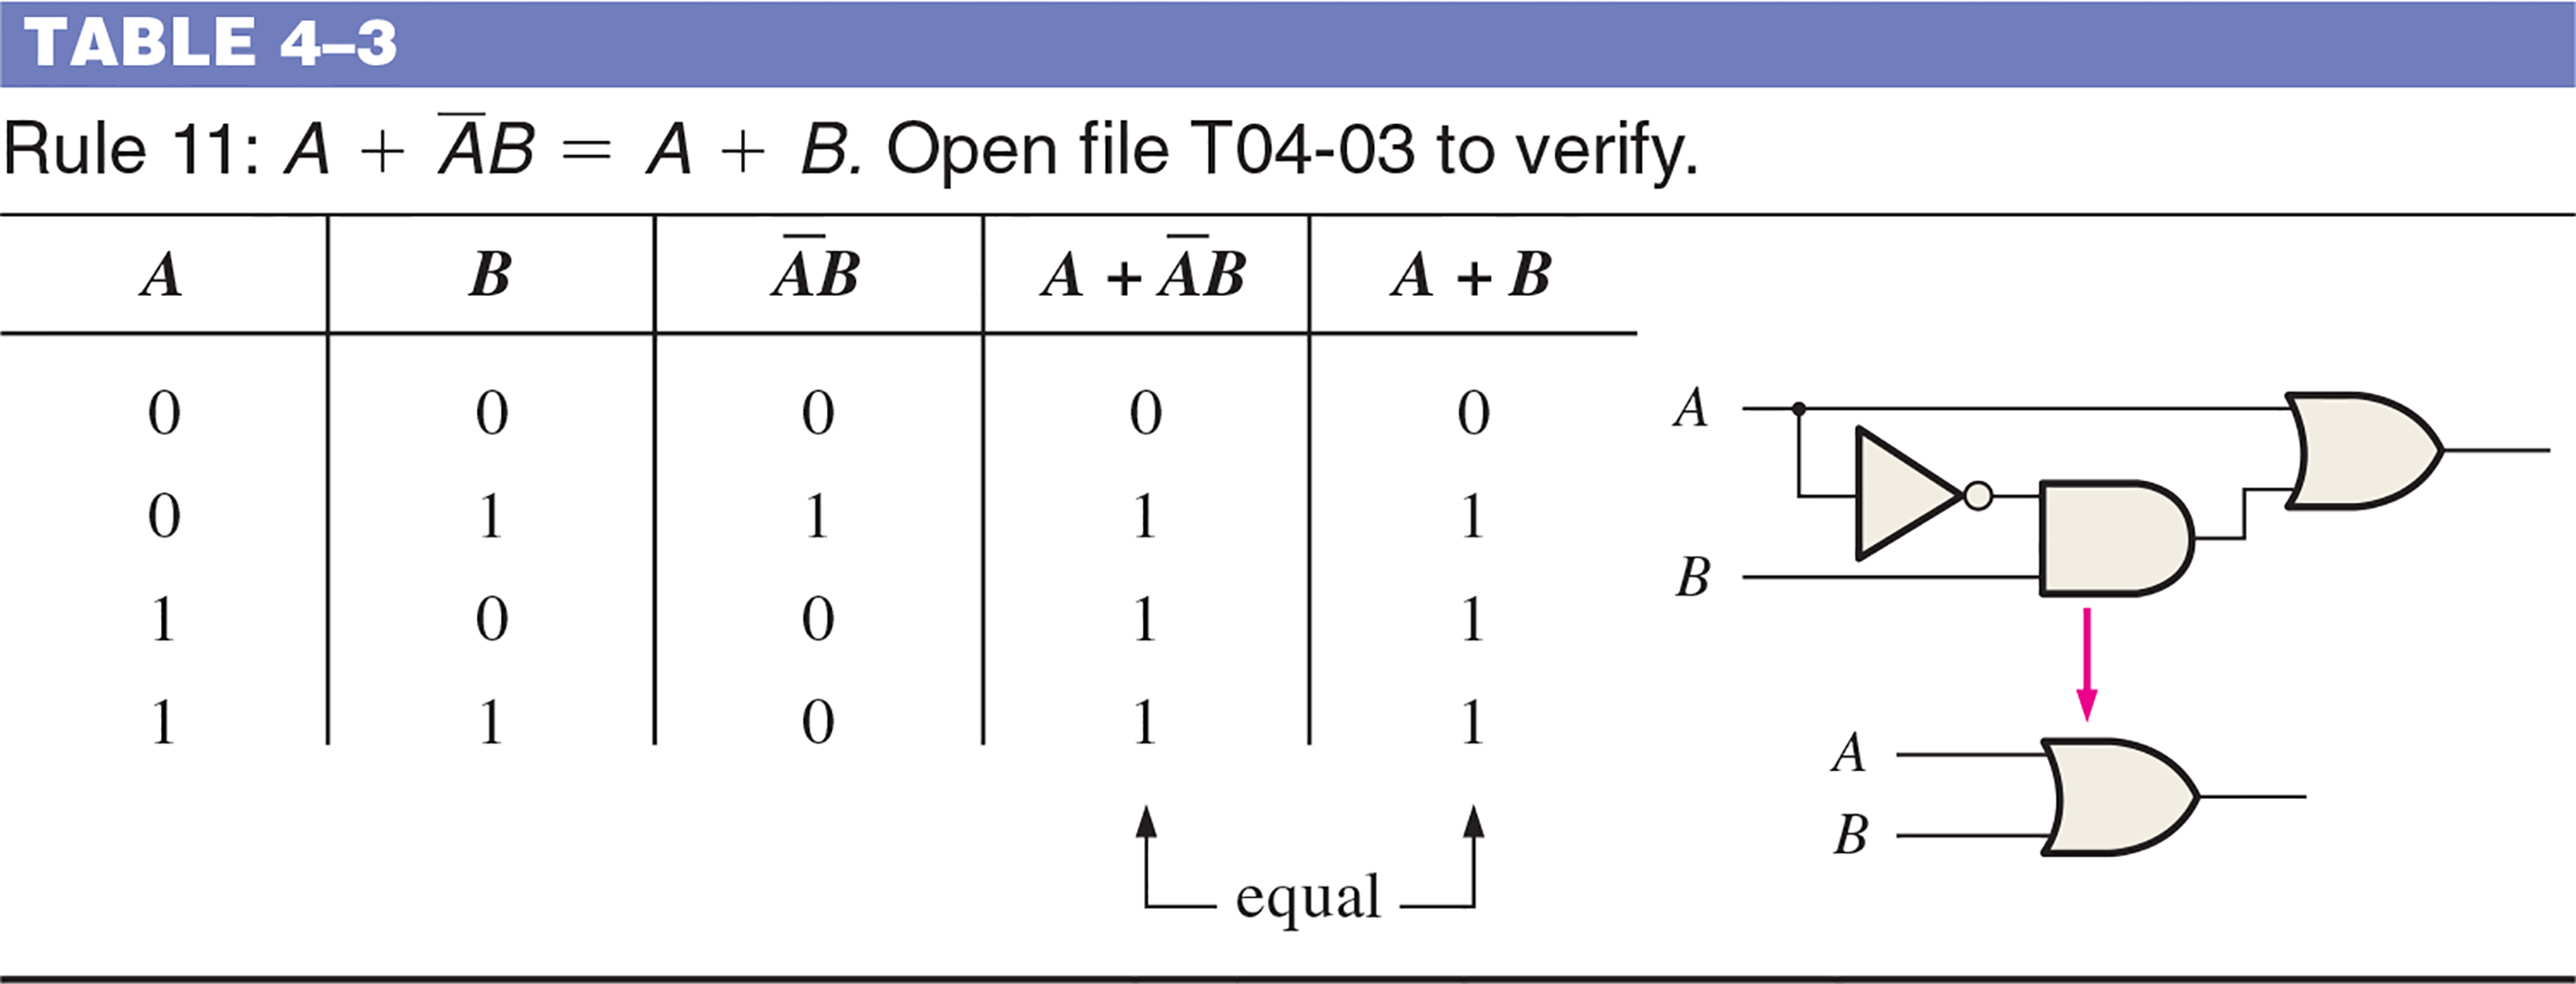
\includegraphics[width=0.33\textwidth,trim=14cm 1cm 0cm 3cm,clip=true]{figures/AND_OR_2.jpg} \hspace{0.5cm}
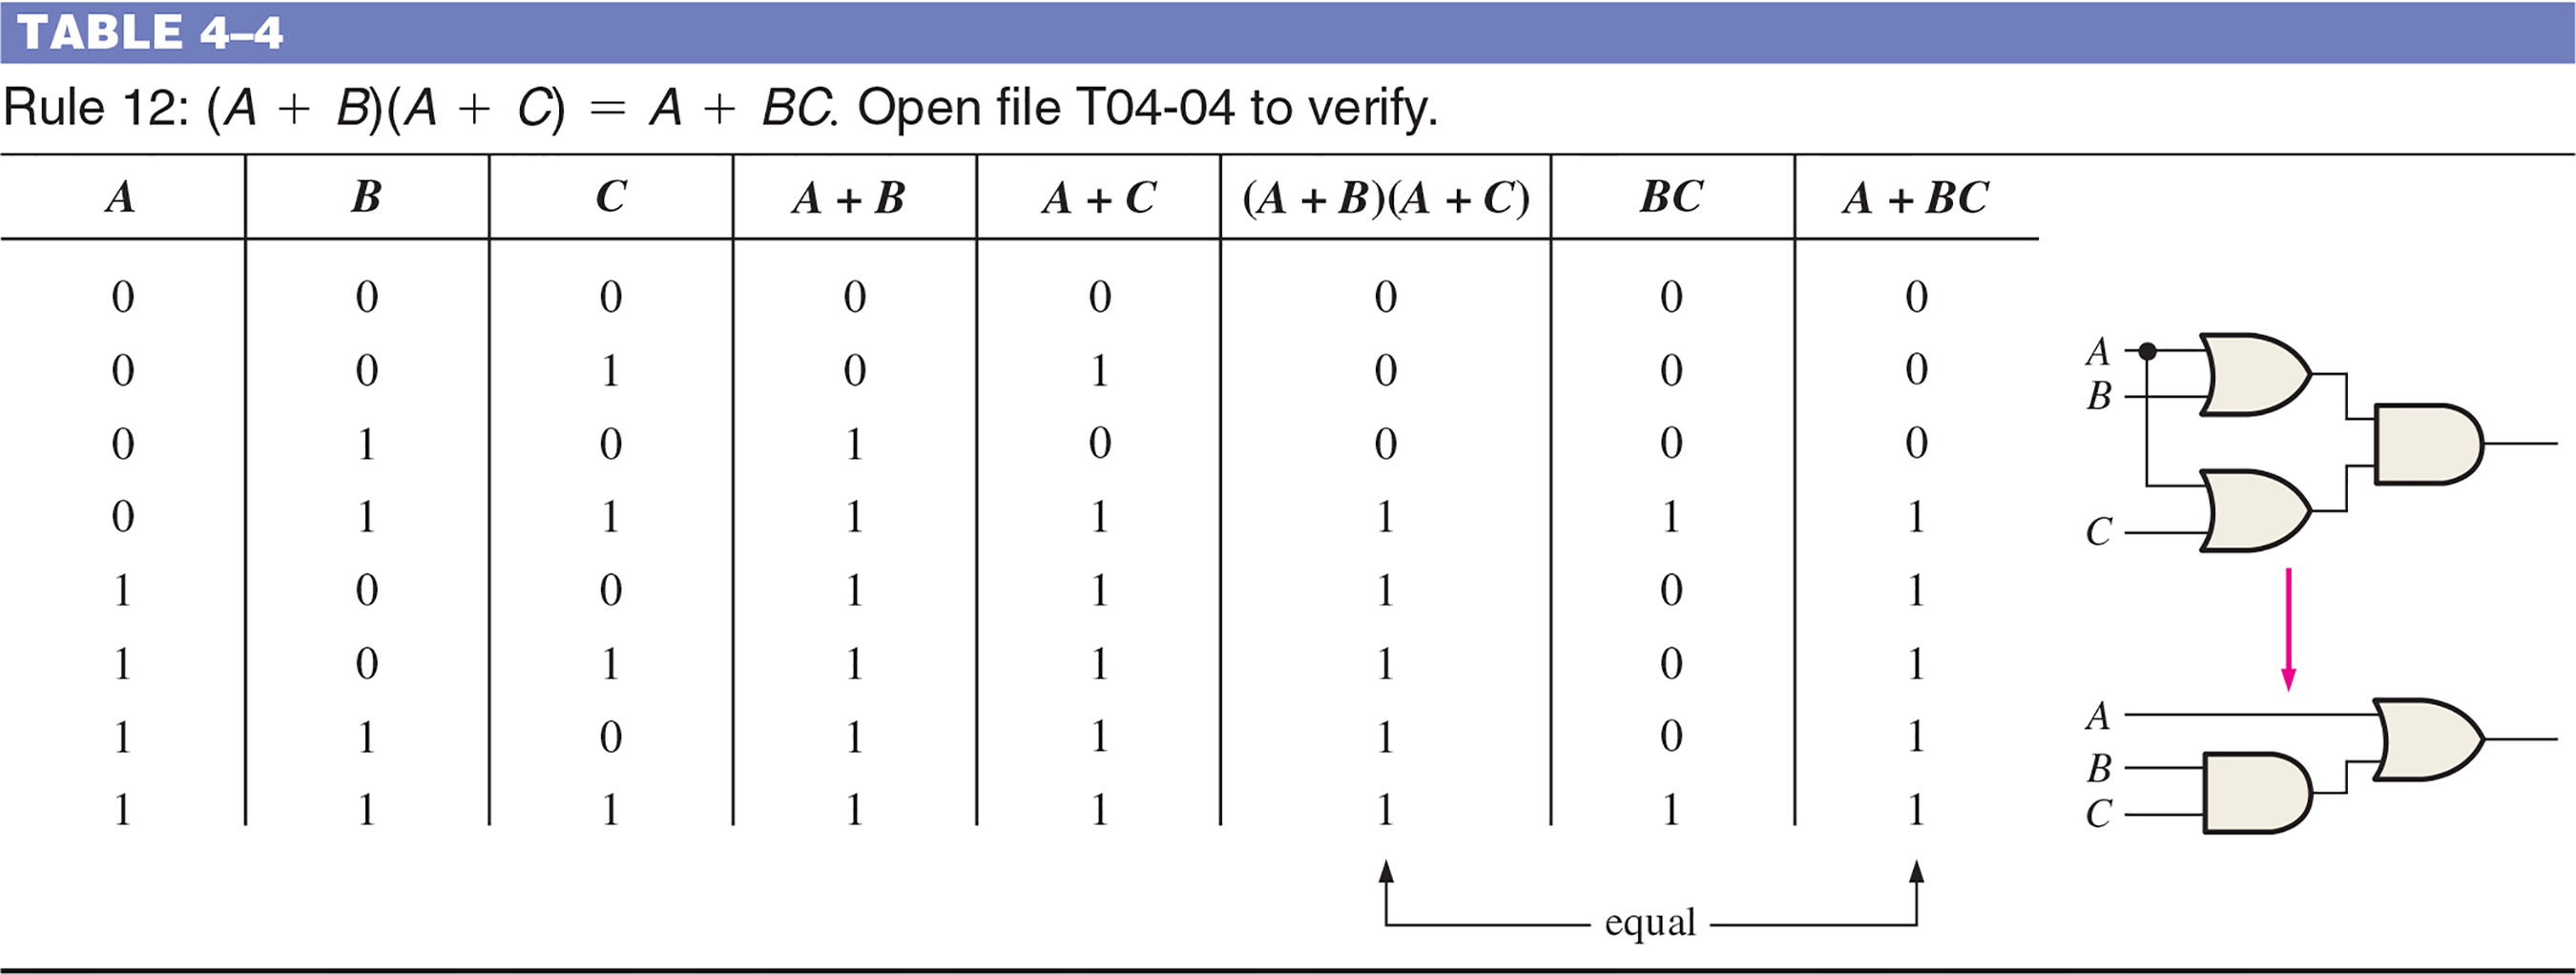
\includegraphics[width=0.25\textwidth,trim=18cm 1cm 0cm 2.5cm,clip=true]{figures/AND_OR_3.jpg}
\caption{\label{fig:and} (a) Show that $A+AB = A$. (b) Show that $A+\bar{A}B = A+B$. (c) Show that $(A+B)(A+C) = A + BC$.}
\end{figure}

\section{Logic Circuits and Boolean Algebra}

\begin{enumerate}
\item Consider the three circuits in Fig. \ref{fig:and}.  Prove that each reduces to a simpler circuit using a truth table. \\ \vspace{2cm}
\item Consider the following equation:
\begin{equation}
X = \overline{\overline{A+B\bar{C}} + D\overline{(E+\bar{F})}}
\end{equation}
(a) Use DeMorgan's Theorems to reduce this expression. (b) Draw a circuit corresponding to the \textit{unsimplified} expression.  (c) Draw a circuit corresponding to the \textit{simplified} expression.  (d) How many gates are removed from the design through simplificiation?
\end{enumerate}

\end{document}
